\part{Teorie}

\chapter{Základní geometrické pojmy}

\section{Přímky a úsečky}

Mějme dva body $x_1, x_2 \in \mathbb{R}^n$ takové, že $x_1 \neq x_2$ a parametr $\theta \in \mathbb{R}^n$. Potom výraz
\begin{equation}
    y = \theta x_1 + (1 - \theta) x_2
    \label{line}
\end{equation}
popisuje \textbf{přímku} procházející body $x_1$ a $x_2$. Pro $\theta = 0$ dostáváme bod $x_2$ a pro $\theta = 1$ bod $x_1$. Omezíme-li $\theta$ na interval $\langle 0, 1 \rangle$, dostaneme \textbf{úsečku} s koncovými body $x_1$ a $x_2$. Výraz \ref{line} lze přepsat do tvaru
$$
    y = x_2 + \theta (x_1 - x_2),
$$
který můžeme interpretovat jako součet počátečního bodu $x_2$ a nějakého násobku směrového vektoru $x_1 - x_2$.

\section{Affiní množiny}

Říkáme, že $C \subseteq \mathbb{R}^n$ je \textbf{afinní množina}, jestliže přímka procházející libovolnými dvěma různými body z $C$ leží v $C$. Tedy $C$ obsahuje lineární kombinace libovolných dvou bodů z $C$, jestliže součet koeficientů lineární kombinace je roven jedné. To lze zobecnit i pro více než dva body. Lineární kombinace $\theta_1 x_1 + \dots + \theta_k x_k$ bodů $x_1, \dots, x_k$ taková, že $\theta_1 + \dots + \theta_k = 1$, se nazývá \textbf{afinní kombinace} bodů $x_1, \dots, x_k$. Indukcí z definice afinní množiny lze snadno ukázat, že pokud $C$ je afinní množina, $x_1, \dots, x_k \in C$ a $\theta_1 + \dots + \theta_k = 1$, potom bod $\theta_1 x_1 + \dots + \theta_k x_k \in C$.

\noindent Nechť $C$ je afinní množina a $x_0 \in C$, potom množina
$$
    V = C - x_0 = \left\{ x - x_0 \mid c \in C \right\}
$$
je \textbf{vektorový prostor}, tj. množina, která je uzavřená na sčítání a násobení skalárem.

\noindent Afinní množinu $C$ lze vyjádřit jako
$$
    C = V + x_0 = \left\{ v + x_0 \mid v \in V \right\},
$$
kde $V$ je vektorový prostor a $x_0$ je počátek. Poznamenejme, že vektorový prostor $V$ asociovaný s afinní množinou $C$ nezávisí na volbě počátku $x_0$.

\noindent \textbf{Dimenze} afinního množiny $C = V + x_0$ je definována jako dimenze vektorového prostoru $V = C - x_0$, kde $x_0$ je libovolný prvek z $C$. Množina všech affiních kombinací bodů množiny $C \subseteq \mathbb{R}^n$ se nazývá \textbf{affiní obal} množiny $C$. Affiní obal množiny $C$ budeme značit
$$
    \textbf{aff } C = \left\{ \theta_1 x_1 + \dots + \theta_k x_k \mid x_1, \dots, x_k \in C, \theta_1 + \dots + \theta_k = 1 \right\}.
$$
Affiní obal je nejmenší affiní množina, která obsahuje množinu $C$. Tedy, jestliže $S$ je affiní množina taková, že $C \subseteq S$, potom $\textbf{aff }C \subseteq S$.


\section{Konvexní množiny}

Říkáme, že množina $C$ je \textbf{konvexní}, jestliže úsečka mezi libovolnými dvěma body z $C$ leží také v $C$. Jinak řečeno, jestliže pro libovolné dva body $x_1, x_2 \in C$ a libovolné $\theta \in \langle 0, 1 \rangle$ platí, že $\theta x_1 + (1 - \theta) x_2 \in C$. Poznamenejme, že každá afinní množina je zároveň konvexní množinou. Podobně jako affiní kombinaci definujeme \textbf{konvexní kombinaci} bodů $x_1, \dots, x_k$ jako $\theta_1 x_1 + \dots + \theta_k x_k$, kde $\theta_1 + \dots + \theta_k = 1, \theta_i \geq 0$ pro $i = 1, \dots, k$. \textbf{Konvexní obal} množiny $C$ je množina všech konvexních kombinací bodů z množiny $C$, značíme
$$
    \textbf{conv }C = \left\{ \theta_1 x_1 + \dots + \theta_k x_k \mid x_i \in C, \theta_i \geq 0, i = 1, \dots, k, \theta_1 + \dots + \theta_k = 1 \right\}.
$$
Analogicky, konvexní obal množiny $C$ je nejmenší konvexní množina, která obsahuje množinu $C$. Pro představu viz obrázek~\ref{fig:convex_hull}.

\begin{figure}[h!]
    \centering
    \begin{subfigure}[b]{0.3\textwidth}
        \centering
        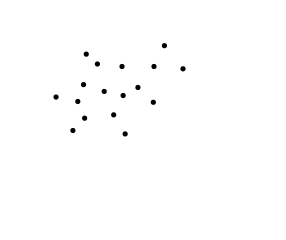
\includegraphics[width=\textwidth]{img/points.png}
        \caption{Množina bodů $C$}
        \label{fig:convex_hull:a}
    \end{subfigure}

    \hfill

    \begin{subfigure}[b]{0.3\textwidth}
        \centering
        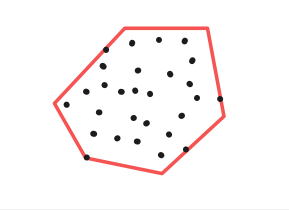
\includegraphics[width=\textwidth]{img/convex_hull.png}
        \caption{$\textbf{conv }C$}
        \label{fig:convex_hull:b}
    \end{subfigure}
     
    \caption{Konvexní obal množiny}
    \label{fig:convex_hull}
\end{figure}


\section{Kužely}

Množina $C$ se nazývá \textbf{kužel}, jestliže pro každé $x \in C$ a $\theta \geq 0$ platí, že $\theta x \in C$. Je-li $C$ navíc konvexní, pak se $C$ nazývá \textbf{konvexní kužel}. Tedy $C$ je konvexní kužel, jestliže pro libovolné $x_1, x_2 \in C$ a $\theta_1, \theta_2 \geq 0$ platí, že $\theta_1 x_1 + \theta_2 x_2 \in C$. Říkáme, že bod ve tvaru $\theta_1 x_1 + \dots + \theta_k x_k$, kde $\theta_1, \dots, \theta_k \geq 0$ je \textbf{kuželovou kombinací} bodů $x_1, \dots, x_k$. Dále, pokud $x_i$ leží v konvexním kuželu množiny $C$, potom libovolná kuželová kombinace bodu $x_i$ leží rovněž v konvexním kuželu množiny $C$. Platí, že množina $C$ je konvexní kužel právě tehdy, když $C$ obsahuje všechny kuželové kombinace svých bodů. \textbf{Kuželový obal} množiny $C$ je množina, která obsahuje všechny kuželové kombinace množiny $C$, tj.
$$
    \left\{ \theta_1 x_1 + \dots + \theta_k x_k \mid x_i \in C, \theta_i \geq 0, i = 1, \dots, k \right\}.
$$
Kuželový obal množiny $C$ je zároveň nejmenší konvexní kužel, který obsahuje množinu $C$. Pro představu viz obrázek~\ref{fig:cone_hull}.

\begin{figure}[h!]
    \centering
    \begin{subfigure}[b]{0.3\textwidth}
        \centering
        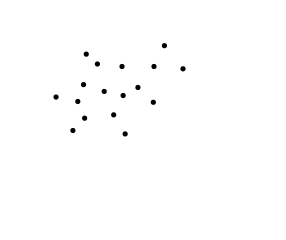
\includegraphics[width=\textwidth]{img/points.png}
        \caption{Množina bodů $C$}
        \label{fig:cone_hull:a}
    \end{subfigure}

    \hfill

    \begin{subfigure}[b]{0.3\textwidth}
        \centering
        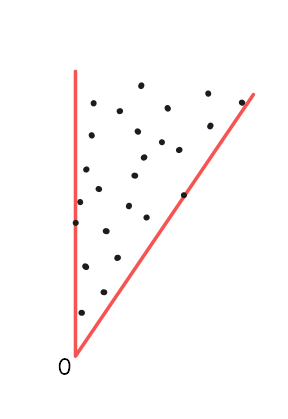
\includegraphics[width=\textwidth]{img/cone_hull.png}
        \caption{$\textbf{conv }C$}
        \label{fig:cone_hull:b}
    \end{subfigure}
     
    \caption{Kuželový obal množiny}
    \label{fig:cone_hull}
\end{figure}

\section{Nadroviny a poloprostory}

\textbf{Nadrovina} je množina ve tvaru
$$
    \left\{ x \mid a^T x = b \right\},
$$
kde $a \in \mathbb{R}^n$, $a \neq 0$ a $b \in \mathbb{R}$. Analyticky se na nadrovinu koukáme jako na množinu všech řešení netriviální lineární rovnice. Geometricky zase jako na množinu všech bodů takových, že mají konstantní skalární součin s normálovým vektorem $a$. Konstanta $b$ značí posunutí nadroviny od počátku. Nadrovinu také můžeme vyjádřit jako
$$
    \left\{ x \mid a^T (x - x_0) = 0 \right\} = x_0 + \left\{ v \mid a^T v = 0 \right\},
$$
kde $x_0$ je libovolný bod této nadroviny a $\left\{ v \mid a^T v = 0 \right\}$ je množina všech vektorů, které jsou kolmé k normálovému vektoru $a$. Nadrovina je tedy množina, která obsahuje bod $x_0$ a libovolný bod ve tvaru $x_0 + v$, kde $v$ je vektor, který je kolmý k normálovému vektoru $a$. Pro ilustraci v $\mathbb{R}^2$ viz obrázek~\ref{fig:hyperplane}.

Nadrovina dělí $\mathbb{R}^n$ na dva poloprostory. Množina 
$$
    \left\{ x \mid a^T x \leq b \right\}, \text{ resp. } \left\{ x \mid a^T x < b \right\},
$$
kde $a \neq 0$ se nazývá (uzavřený) \textbf{poloprostor}, resp. \textbf{otevřený poloprostor}. Je to tedy množina všech řešení netriviální lineární nerovnice. Podobně jako nadrovinu, můžeme poloprostor vyjádřit ve tvaru
$$
    \left\{ x \mid a^T (x - x_0) \leq 0 \right\}, \text{ resp. } \left\{ x \mid a^T (x - x_0) < 0 \right\},
$$
kde $a \neq 0$ a $x_0$ je libovolný bod z nadroviny $\left\{ x \mid a^T x = b \right\}$. Poloprostor tedy obsahuje bod $x_0$ a libovolný bod $x_0 + v$, kde $v$ je vektor, který s vnějším normálovým vektorem svírá tupý nebo pravý úhel. Tato interpretace je v $\mathbb{R}^2$ ilustrována na obrázku~\ref{fig:halfspace}. Ještě poznamenejme, že poloprostory jsou konvexní množiny, ale samozřejmě nejsou affiní.

\begin{figure}[h!]
    \centering
    \begin{subfigure}[b]{0.3\textwidth}
        \centering
        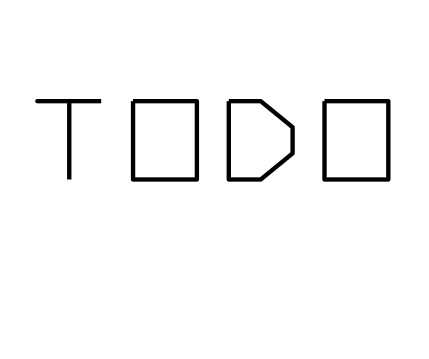
\includegraphics[width=\textwidth]{img/todo.png}   
        \caption{Nadrovina}
        \label{fig:hyperplane}
    \end{subfigure}

    \hfill

    \begin{subfigure}[b]{0.3\textwidth}
        \centering
        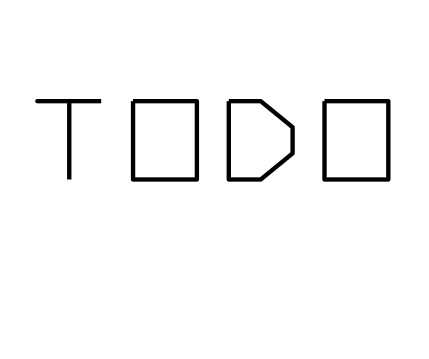
\includegraphics[width=\textwidth]{img/todo.png}   
        \caption{Poloprostor}
        \label{fig:halfspace}
    \end{subfigure}

    \caption{Nadrovina a poloprostor v $\mathbb{R}^2$.}
    \label{fig:hyperplane_halfspace}
\end{figure}

\section{Polyedry a polytopy}


\chapter{Lineární programování}

\section{Formulace úlohy}

Úlohou lineárního programování rozumíme minimalizaci nebo maximalizaci lineární \textbf{účelové funkce} vzhledem k lineárním \textbf{omezením}, kde tato omezení mohou být dána soustavou lineární rovnic a nerovnic. Úlohu lineárního programování lze formulovat v několika tvarech, které se liší zadáním omezení. Úloha lineárního programování ve \textbf{standardním tvaru} má svá omezení dána soustavou lineárních rovnic $Ax = b$. Tedy
\begin{equation}
    \min \left\{ c^T x \mid Ax = b, x \geq 0 \right\}, \tag{LP-P}
    \label{eq:LP-P}
\end{equation}
kde $A \in \mathbb{R}^{m \times n}$, $b \in \mathbb{R}^n$, $x \in \mathbb{R}^n$ a $c \in \mathbb{R}^n$. \textbf{Přípustná množina řešení} je průnikem affiního prostoru, který je definován soustavou rovnic $Ax = b$ a \textbf{nezáporného ortantu}, tj. množiny $\left\{ x \in \mathbb{R}^n \mid x_i \geq 0, i = 1, \dots, n \right\}$. Obě tyto množiny jsou konvexní a tedy i jejich průnik je rovněž konvexní množina. Dále, protože přípustnou množinu máme popsanou soustavou konečně mnoha lineárních rovnic a nerovnic, geometricky se na úlohu \ref{eq:LP-P} můžeme koukat jako na minimalizaci lineární funkce přes polyedr, který je definován touto soustavou. 

\section{Dualita}

\section{Komplementární skluzovost}

\chapter{Semidefinitní programování}
%spektraedr, formulace, dualita, semidefinitní kužel, duální kužel, ...
%vektorové programování a jeho ekvivalence, formulace úloh

\chapter{Kuželové programování}
%jen stručně pro úplnost
